%----------------------------------------------------------------------------------------
%	PACKAGES AND OTHER DOCUMENT CONFIGURATIONS
%----------------------------------------------------------------------------------------

\documentclass[12pt]{article} % Default font size is 12pt, it can be changed here

\usepackage[margin=1in]{geometry} % Required to change the page size to A4
\geometry{a4paper} % Set the page size to be A4 as opposed to the default US Letter

\usepackage{graphicx} % Required for including pictures

\usepackage{float} % Allows putting an [H] in \begin{figure} to specify the exact location of the figure
\usepackage{wrapfig} % Allows in-line images such as the example fish picture

\usepackage{hyperref}
\usepackage{microtype}
\microtypesetup{protrusion=true} % enables protrusion
\linespread{1.2} % Line spacing

%\setlength\parindent{0pt} % Uncomment to remove all indentation from paragraphs

\graphicspath{{Pictures/}} % Specifies the directory where pictures are stored

\begin{document}

%----------------------------------------------------------------------------------------
%	TITLE PAGE
%----------------------------------------------------------------------------------------

\begin{titlepage}

\newcommand{\HRule}{\rule{\linewidth}{0.5mm}} % Defines a new command for the horizontal lines, change thickness here

%\center % Center everything on the page

  \begin{flushright}
    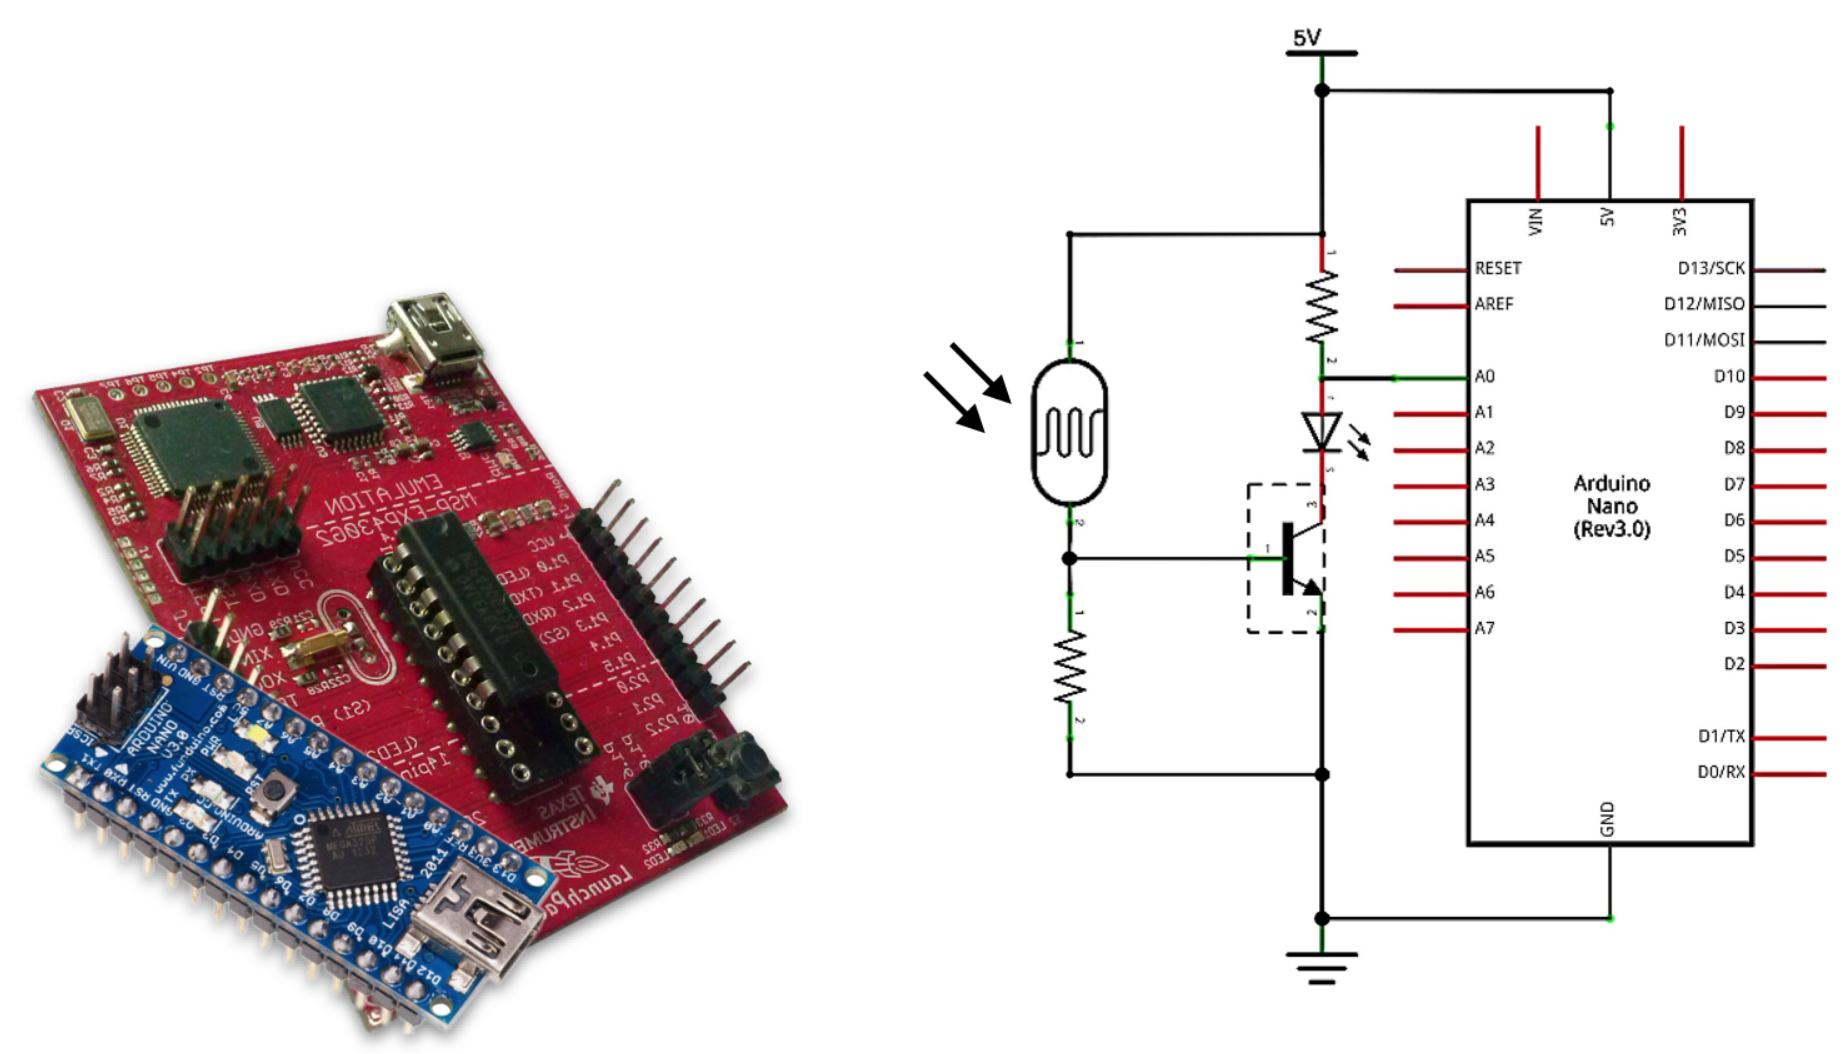
\includegraphics[width=0.7\textwidth]{banner2}
  \end{flushright}

\vspace{30 mm}

\textsc{\large A workshop}\\ % Name of your university/college

%\HRule \\[0.4cm]
{ \huge \bfseries Embedded Systems Made Easy}\\[0.4cm] % Title of your document

\begin{minipage}{0.4\textwidth}
\begin{flushleft}
Sanjeet Raj \textsc{Pandey}\\ 
Technical University Berlin\\ 
\textsc{Germany}\\ 
Workshop@lifemachine.net\\
\end{flushleft}
\end{minipage} \\[5cm]

\begin{minipage}{0.4\textwidth}
\begin{flushleft}
\emph{\large Date and Venue:}\\
\large 10 - 11 March 2014\\
Hotel Manaki, Janakpur\\ 
\textsc{Nepal}\\ 
\end{flushleft}
\end{minipage}

\vfill % Fill the rest of the page with whitespace

\end{titlepage}

%----------------------------------------------------------------------------------------
%	TABLE OF CONTENTS
%----------------------------------------------------------------------------------------
% not needed, i think, or sanjeet??
%\tableofcontents % Include a table of contents

%\newpage % Begins the essay on a new page instead of on the same page as the table of contents 

%----------------------------------------------------------------------------------------
%	Motivation
%----------------------------------------------------------------------------------------

\section{Motivation} % Major section
Advancement in technology needs a careful and continuous following. Mobile systems, broadcasting methods, medical machinery are few technologies without which life is hard to imagine. Technology is leading the frontiers from saving lives, security, defense, and space exploration to mundane aspects as entertainment or social networking. Electronics, than ever before, is vital part of any society now.\vspace{1mm}

Big industries are investing millions to get innovative application out of Embedded Systems today, they also, however, have started a culture of patents and closed sources. On the other hand, Homebrew, Do It Yourself (DIY) and Open Source are playing important role to keep these technologies transparent and accessible. \vspace{1mm}

Open Source Hardware and Software have massively improved in the quality, user experience and have become more affordable to buy. We are motivated to promote this experience to school students and enthusiasts; introduce them the possibilities beyond simple transistor circuits and facilitate them venture into the embedded systems.\vspace{1mm}

A do it yourself workshop on embedded electronics and applications is an initiative with following key ideas:

\begin{itemize}
\item How simple and easy it is
\item Think beyond
\item Internet of things
\item Cheaper hardware
\item Coding has never been easier
\item Understanding how complex devices work \ldots
\end{itemize}

\section{Programme} % Program flow
The main agenda is learning by making, therefore, maximum time is assigned for DIY sessions.
\begin{enumerate}
\item Each session can have maximum of 10 groups with 2 students per sub-group
\item Each session spans for 4 hour
\item First 30 Minutes will be for basic introduction of:  
	\begin{itemize}
		\item Basic electronic components (LED, Resistor, Relay, Transistor)
		\item Microcontroller
		\item Basic C coding
	\end{itemize}
\item Do It Yourself (DIY) session for 3.5 hour with different projects:
	\begin{itemize}
	\item Blink LEDs, Switching and reading Analog signals
	\item Reading temperature value
	\item Magnetic switch
	\item Light sensing
	\item Motor driver
	\end{itemize}
\item Demonstration of some finished projects, as, SMS controlled Lights, RGB Lighting
\item Link will be provided prior to Workshop for software along with related documentation.
\item There will be also an open discussion at the end of the programme. Participants are encouraged to interact and pose questions
\end{enumerate}

\section{Session description} % Program flow
Due to Limited supply of hardware/components, sessions are conducted in groups with a question-answer session at the end.
\begin{enumerate}
\item Each session will have maximum of 20 students forming 10 groups.
\item Each session is dedicated to one institution only.
\item There will be a list of different projects. Each group selects a project from this list.  
\item Each group gets a Hardware Kit pre connected to PC 
\item Groups can bring their own laptop, this is highly recommended. 
	\begin{itemize}
	\item Can save project data
	\item Software can be pre installed to save time
	\item Latest OS (tested on windows 7,8, Ubuntu 12.04 or higher, OSX)
	\end{itemize}
\item Participants must abide by basic discipline and be supportive of the event and other groups. Participants who disturb others or violate social discipline will be irrefutably disqualified.
\end{enumerate}

\section{Requirements} % Requiremets
We are delivering main hardware kits from outside of Nepal (Germany), therefore, participating institutions should cover their own expenses. Each hardware kit contains a complete set of components to begin with basic micro-controller circuits. The calculated price for each hardware kit is Rs.8800. Hardware Kit will be distributed after the workshop. We hope that:
\begin{itemize}
\item Each participating institution could buy 3 to 5 hardware kit.
\item Institutions may choose to participate without purchasing the hardware kit for Rs. 3500.
\end{itemize}
The basic raw material cost of these kits is Rs. 8800. The participating institution's willingness to buy these kits will help us finance the workshop. It will also be beneficial for their students to gain more hands on experience with these equipment.\footnote{Minimum calculated cost of each kit is Rs 8800. This is the least  possible cost. We neither have control over this prices nor  we intend to make any profit out of it. }


\subsection{Online registration} % requirementssub
Participating students are encouraged to visit the page \url{http://lifemachine.net/}. Here, the participants can find the source codes to program the micro-controllers, programming IDE and documentations. The online registration form can also be found on the website.

We encourage the individual students to \textbf{register online}. This will help us keep track of the students and copies of the needed software and hardware we have to distribute. This will also be helpful to keep record of their progress and communicate with them in future in case they are willing to learn more or want some help.

\section{Future possibilities} % Requiremets
After the completion of workshop, students will have working knowledge of Embedded Systems, programming them, designing new projects and using them. Here are few popular topics that will that will be introduced as potential projects:
\begin{enumerate}
\item Basic Robotics, i.e. motor control, digital switching and sensing
\item Sensors, Temperature Alarm Systems, Distance measurement, and Reed Switch
\item LED, Dimmers, Optical electronics i.e. LCD, Touch Sensing etc.
\item Power Regulation, AC switching
\item Radio and wireless
\item Binding things to internet  
\item BUS systems (SPI, $I^2C$, 1-Wire etc.)
\item DIY Gadgets
\item Data Logging
\item GPS Sensing
\item Advanced Hardware and Microcontroller (ARM and Higher AVR)
\end{enumerate}
\vspace{0.5cm}
%------------------------------------------------
\emph{\large “Skill to do comes of doing”}\\
\textsc {Ralph Waldo Emerson}

\section*{References} % The bibtex has some trouble, so temporarily i put the references in crappy way
\begin{enumerate}
\item \url{http://lifemachine.net/}
\item \url{http://www.atmel.com/devices/ATMEGA328P.aspx}
\item \url{http://www.raspberrypi.org/}
\item \url{http://processors.wiki.ti.com/index.php/MSP430_LaunchPad_(MSP-EXP430G2)}
\item \url{http://arduino.cc/en/Main/ArduinoBoardMicro}
\item \url{http://www.pjrc.com/teensy/}
\item \url{http://www.tkn.tu-berlin.de/}
\end{enumerate}


\section*{Special Thanks to}
\begin{itemize}
\item Prof. Dr.-Ing. Adam Wolisz , Telecommunication Networks Group , TU-Berlin
\item Dr.-Ing.Vlado Handziski , Telecommunication Networks Group , TU-Berlin
\item Felix Schaal , Berlin Promotion Agency, Berlin
\item Nepalese Students Society in Germany
\end{itemize}


\end{document}